\documentclass[journal=jctcce,manuscript=article]{achemso}

\usepackage{graphicx}
\usepackage{booktabs}
\usepackage{amsmath}
\usepackage{hyperref}

\title{Why Local ML Models Cannot Accelerate SCF Convergence
in Multiresolution Analysis: Lessons from Systematic Architecture Search}

\author{Ruhin Patel}
\email{ruhinrakeshkum.patel@stonybrook.edu}
\affiliation{Department of Applied Mathematics and Statistics, Stony Brook University, Stony Brook, NY 11794}
\author{Adrian Hurtado}
\email{adrian.hurtado@stonybrook.edu}
\affiliation{Institute for Advanced Computational Science, Stony Brook University, Stony Brook, NY 11794}
\author{Robert J.~Harrison}
\email{robert.harrison@stonybrook.edu}
\affiliation{Department of Applied Mathematics and Statistics, Stony Brook University, Stony Brook, NY 11794}
\affiliation{Institute for Advanced Computational Science, Stony Brook University, Stony Brook, NY 11794}

\begin{document}

\begin{abstract}
We present a systematic investigation of machine learning approaches
to accelerating self-consistent field (SCF) convergence in MADNESS,
a multiresolution analysis (MRA) framework for density functional
theory. Using a FiLM-conditioned MLP with same-level halo neighbors
(MRANet, 3.0M parameters), we trained on 51 W4-11 molecules and
evaluated three strategies: density coefficient prediction, parent
node augmentation, and tree structure prediction. The density
predictor achieved MSE ratios of 0.41--0.98$\times$ baseline at
fine tree levels (10--14) but 1.00--1.12$\times$ at coarse levels
(1--9), where SCF convergence is determined. Injecting the predicted
density into MADNESS produced identical SCF iteration counts across
all 14 molecule-threshold combinations tested. Parent node features
(4.1M parameters) did not change the coarse-level ratios. A
refinement classifier reached F1\,=\,0.860 but increased SCF
iterations 2.6$\times$. All three strategies hit the same limit:
at coarse tree levels, the promolecular density and nuclear potential
do not encode the electron-electron interactions needed for density
corrections. We extract three transferable lessons for ML applied to
multi-scale iterative solvers and propose Gaussian-basis densities as
a richer input signal.
\end{abstract}

\section{Introduction}\label{sec:introduction}

MADNESS~\cite{harrison2016madness} is a multiresolution analysis (MRA) framework for density functional theory that represents functions as adaptive octree structures of polynomial scaling coefficients.
The tree refines locally where the function has fine-scale features and remains coarse elsewhere, achieving systematic accuracy without a fixed basis set.
Within a MADNESS DFT calculation, self-consistent field (SCF) iteration dominates wall time: each iteration rebuilds the Coulomb and exchange-correlation potentials, solves the bound-state Helmholtz equation for every orbital, and updates the density.
The standard initial density guess is the promolecular density $\rho_0$, a superposition of isolated spherical atomic densities.
Because $\rho_0$ contains no bonding, charge transfer, or exchange-correlation information, the SCF procedure typically requires 8--15 iterations to converge.
A more accurate starting density would reduce the iteration count and, proportionally, the total cost.

Machine learning models for electron density prediction have shown that neural networks can map nuclear geometry to real-space charge densities with useful accuracy~\cite{gong2025gedcrn}.
These approaches typically predict density on fixed Cartesian grids and project the result onto whatever basis the solver requires.
Working directly in the native MRA representation sidesteps grid-to-tree projection and preserves the adaptive structure that makes MADNESS efficient.
The octree further decomposes the prediction problem into per-node regression tasks with local spatial context available from same-level neighbor nodes, a natural inductive bias for an MLP architecture.

We present a systematic investigation of three ML strategies for accelerating SCF convergence in MADNESS: direct prediction of converged density coefficients, parent-augmented coefficient prediction, and tree structure (refinement) prediction.
All three use a FiLM-conditioned MLP (MRANet) with same-level halo neighbor features as input.
Despite strong per-node regression accuracy at fine tree levels, none of the strategies reduced SCF iteration count when the predicted density was used as an initial guess.
We trace this failure to an input signal bottleneck: at the coarse tree levels that determine SCF convergence behavior, the promolecular density $\rho_0$ and nuclear potential $V_\mathrm{nuc}$ lack the electron-electron interaction information needed to predict density corrections.
The model learns an accurate identity mapping at fine levels (where $\rho_0 \approx \rho$) but cannot extract the missing physics at coarse levels.
From this negative result we extract three lessons transferable to ML applied to multi-scale iterative solvers: (1) input signal quality at the scale that matters for the solver sets the model ceiling, regardless of aggregate accuracy; (2) fine-level accuracy does not imply solver acceleration; and (3) multi-task interference between level-dependent objectives can silently degrade training.

\section{Background}\label{sec:background}

\subsection{Multiresolution Analysis in MADNESS}\label{sec:mra}

MADNESS~\cite{harrison2016madness} represents three-dimensional functions in a discontinuous multiwavelet basis built on an adaptive octree.
The simulation cell $[0,1)^3$ is recursively bisected along each axis to produce cubic boxes at integer levels $n = 0, 1, 2, \ldots$, with each box at level $n$ identified by a translation index $\mathbf{l} \in \{0, \ldots, 2^n - 1\}^3$.
Within each box, the function is expanded in a tensor product of Legendre scaling polynomials of order $k$ (we use $k = 8$ throughout), giving $k^3 = 512$ scaling coefficients (s-coefficients) per node.

The connection between consecutive levels is mediated by Alpert's two-scale relation~\cite{alpert1993twoscale}.
A parent node's s-coefficients can be decomposed into the s-coefficients of its eight children plus a set of wavelet difference coefficients (d-coefficients) that encode the detail lost in the coarsening.
Refinement is controlled by the d-coefficient norm: if $\|\mathbf{d}\| > \epsilon$ for a prescribed threshold $\epsilon$, the node is subdivided into eight children and the representation is extended to the next level.
Nodes whose d-coefficients fall below $\epsilon$ become leaves.
This adaptive refinement concentrates computational effort near nuclei and in bonding regions while keeping the representation coarse in smooth, slowly varying parts of space.

\subsection{SCF Iteration Mechanics}\label{sec:scf}

Kohn-Sham DFT~\cite{kohn1965self} reduces the many-electron problem to a set of single-particle eigenvalue equations in which the effective potential depends on the electron density $\rho(\mathbf{r})$.
Because the potential is a functional of $\rho$, the equations must be solved self-consistently: an initial density defines a potential, the eigenvalue equations are solved for new orbitals, a new density is constructed, and the cycle repeats until $\rho$ changes by less than a convergence threshold.

MADNESS uses the promolecular density $\rho_0(\mathbf{r}) = \sum_A \rho_A^\mathrm{atom}(\mathbf{r})$ as its initial guess, where $\rho_A^\mathrm{atom}$ is the spherically symmetric ground-state density of isolated atom $A$.
This superposition is inexpensive to construct and places charge in roughly the right spatial regions, but it contains no information about chemical bonding, charge redistribution, or exchange-correlation effects.
The distance between $\rho_0$ and the converged $\rho$ determines how many SCF iterations are needed.

MADNESS employs a multi-protocol convergence strategy~\cite{harrison2016madness}.
The calculation begins at a coarse truncation threshold (typically $\epsilon = 10^{-4}$), producing a shallow tree with fewer nodes.
Once the density converges at this threshold, the tree is refined to a tighter threshold ($\epsilon = 10^{-6}$ or beyond) and iteration continues.
The first (coarsest) protocol dominates the total iteration count because it starts from $\rho_0$, the density furthest from the converged solution.
Subsequent protocols start from an already-converged density at the previous threshold and typically converge in one or two iterations.
Any ML model that aims to reduce SCF cost must therefore improve the density at coarse levels, where the first protocol operates and where the gap between $\rho_0$ and $\rho$ is largest.

\section{Methods}\label{sec:methods}

\subsection{Data Pipeline}\label{sec:data-pipeline}

Training data was generated from DFT calculations on 51 closed-shell molecules drawn from the W4-11 thermochemistry benchmark set~\cite{karton2011w411}, spanning atomic species H, C, N, O, F, S, and Cl. All calculations used the LDA functional with MADNESS~\cite{harrison2016madness} multiresolution parameters $k=8$ (polynomial order) and $\epsilon = 10^{-6}$ (truncation threshold), matching production precision for the adaptive tree representation.

For each molecule, three MADNESS functions were generated in a three-step pipeline. First, \texttt{dump\_training\_functions} produced the superposition-of-atomic-densities initial guess $\rho_0(\mathbf{r})$ and the nuclear potential $V_\mathrm{nuc}(\mathbf{r})$ as MRA function trees serialized to HDF5. Second, \texttt{moldft} ran the SCF cycle to convergence. Third, \texttt{dump\_training\_functions -{}-archive} extracted the converged density $\rho(\mathbf{r})$ from the moldft checkpoint and wrote it as a third HDF5 tree. Each function is stored as a tree of $k^3 = 512$-element coefficient vectors (the \emph{s-coefficients}) at each node.

\paragraph{Sample construction.}
The dataset builder enumerates every node in the converged $\rho$ tree. Internal nodes (those with children) are labeled as positive samples requiring further refinement (\texttt{refine}=1); leaf nodes are positive samples that do not require refinement (\texttt{refine}=0). To provide negative examples, the builder generates the eight octree children below each leaf node by evaluating $\rho$'s s-coefficients at the child level via the two-scale relation (these children have vanishing wavelet coefficients by construction). The negative samples are labeled \texttt{refine}=0.

For each sample, the input features consist of (i) the $\rho_0$ and $V_\mathrm{nuc}$ s-coefficients at the box itself (each $k^3 = 512$ elements), (ii) the s-coefficients of $\rho_0$ and $V_\mathrm{nuc}$ at six face-adjacent halo boxes (each $6 \times 512$), and (iii) the integer tree level $n$. Halo s-coefficients for neighbors outside the simulation cell are zero-padded. The target is the converged $\rho$ s-coefficient vector at the same box. The complete HDF5 layout stores these arrays per molecule with gzip compression.

\paragraph{Train/val/test split.}
The 51 molecules were split by molecule: 45 for training, 3 for validation (ethanol, SO$_2$, HNNN), and 3 for testing (H$_2$O$_2$, C$_2$H$_2$, glyoxal). This molecule-level split ensures that the validation and test sets probe generalization to unseen geometries and electronic structures, not merely interpolation within a known tree. The 45 training molecules produced approximately 108,000 positive samples.

\subsection{Architecture (MRANet)}\label{sec:architecture}

MRANet is a FiLM-conditioned multilayer perceptron with a factored halo encoder (Figure~\ref{fig:architecture}).

\begin{figure}[htbp]
  \centering
  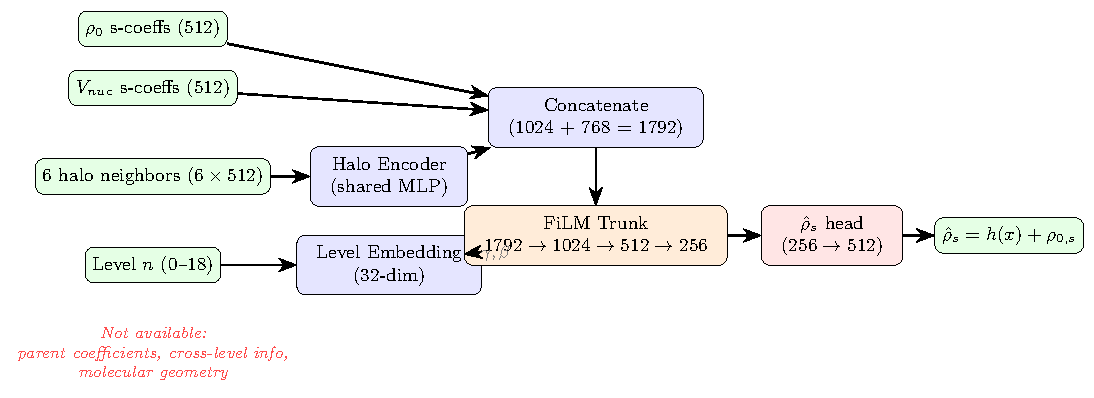
\includegraphics[width=\columnwidth]{figures/fig1_architecture.pdf}
  \caption{MRANet architecture. The model receives $\rho_0$ and $V_\mathrm{nuc}$ s-coefficients at the center box and six face-adjacent halo boxes, conditioned on the tree level via FiLM modulation. A residual connection adds the input $\rho_0$ coefficients to the network output.}
  \label{fig:architecture}
\end{figure}

\paragraph{Halo encoder.}
A shared MLP processes each of the six face-adjacent neighbor boxes identically. Each face's input is the concatenation of the neighbor's $\rho_0$ s-coefficients (512), $V_\mathrm{nuc}$ s-coefficients (512), and a learnable face embedding (8-dimensional, distinguishing $\pm x$, $\pm y$, $\pm z$ faces), giving an input dimension of 1032. The shared MLP maps this to a 128-dimensional output via one hidden layer of 256 units with ReLU activation. The six per-face outputs are concatenated to produce a 768-dimensional halo representation.

\paragraph{Center features.}
The s-coefficients of $\rho_0$ and $V_\mathrm{nuc}$ at the box itself are concatenated into a 1024-dimensional center feature vector.

\paragraph{FiLM conditioning.}
The tree level $n \in \{0, \ldots, 18\}$ indexes a 32-dimensional learned embedding table. At each trunk layer, a linear projection maps this embedding to a per-neuron scale $\gamma$ and shift $\beta$, applied after batch normalization following the FiLM mechanism~\cite{perez2018film}:
\begin{equation}
  \mathbf{h} = \gamma \odot \mathrm{BN}(W\mathbf{x} + \mathbf{b}) + \beta.
\end{equation}
This allows the network to adapt its behavior to the characteristic length scale and coefficient magnitude at each tree level without dedicating separate parameters per level.

\paragraph{Trunk.}
The halo representation and center features are concatenated into a 1792-dimensional input vector, which passes through three FiLM-conditioned layers with dimensions $1792 \to 1024 \to 512 \to 256$. Each layer applies a linear transformation, batch normalization, FiLM modulation, ReLU activation, and dropout ($p = 0.1$) in sequence.

\paragraph{Output head.}
A single linear layer maps the 256-dimensional trunk output to a 512-dimensional vector of predicted $\rho$ s-coefficients. The output uses a residual connection to the input $\rho_0$ s-coefficients:
\begin{equation}
  \hat{\rho}_s = f_\theta(\mathbf{x}) + \rho_{0,s},
\end{equation}
so the network learns the correction $\rho_s - \rho_{0,s}$ rather than the full density. This inductive bias reflects the physical expectation that the converged density is close to the atomic superposition guess. The single-task model contains approximately $3.04 \times 10^6$ parameters.

\subsection{Training and Inference}\label{sec:training}

\paragraph{Loss function.}
The single-task model was trained with a weighted mean squared error loss on the s-coefficient vector. To counteract the class imbalance (approximately 87\% negative samples in the dataset), positive (in-tree) samples received a weight of 10 relative to negative (below-leaf) samples. The loss also incorporated level-aware masking: tree levels with fewer than 200 training samples were excluded entirely (hard cutoff), and the remaining levels were weighted by $\sqrt{c_\ell / c_\mathrm{max}}$ where $c_\ell$ is the sample count at level $\ell$ and $c_\mathrm{max}$ is the maximum count across levels. This soft weighting prevented data-sparse levels from dominating the gradient.

\paragraph{Optimization.}
The model was trained with AdamW (learning rate $2 \times 10^{-4}$, weight decay $10^{-4}$) using a linear warmup over 5 epochs followed by cosine decay to a minimum learning rate of $10^{-6}$. Batch size was 4096 samples. Training used automatic mixed precision (AMP) with gradient scaling and ran for up to 120 epochs with early stopping (patience 20 epochs, monitored on validation loss).

\paragraph{Single-task inference.}
At inference time, \texttt{predict\_density\_simple()} copies the $\rho_0$ tree topology (preserving internal node structure and leaf set), replaces each leaf's s-coefficients with the model's prediction, then runs a compress-reconstruct pass to enforce two-scale consistency throughout the tree. The predicted tree is then scaled so that $\int \hat{\rho}(\mathbf{r})\,d\mathbf{r} = N_e$. Level clamping restricts model predictions to levels 10--14 (where training data is abundant), falling back to unmodified $\rho_0$ coefficients at all other levels.

\paragraph{SCF integration.}
The predicted density was injected into MADNESS's SCF solver as a replacement initial guess. The integration required three components: (i) a C++ modification to \texttt{SCF::initial\_guess()} in \texttt{SCF.cc} (approximately 20 lines) that detects a \texttt{rhoML} archive at startup, loads it via \texttt{ParallelInputArchive}, and rescales to the correct electron count, falling back to the standard $\rho_0$ if the archive is absent; (ii) an \texttt{h5\_to\_archive} converter that reads the HDF5 function tree produced by Python-side inference and writes a MADNESS binary archive compatible with the C++ reader; and (iii) a driver script that runs ML inference, converts the output, and launches \texttt{moldft} with the ML-derived initial guess alongside a baseline run for comparison.

\section{Experiments and Results}
\label{sec:results}

We evaluate the MRANet model in four experiments, each probing a different
hypothesis about why local ML predictions might accelerate SCF convergence.
Training uses 51 molecules from the W4-11 dataset~\cite{karton2011w411}
(45 train, 3 validation, 3 test) at MADNESS production settings ($k=8$,
$\epsilon=10^{-6}$).

\subsection{Density Coefficient Prediction}
\label{sec:density_prediction}

Our first model used multi-task training with Kendall
uncertainty-weighted loss~\cite{kendall2018multitask} to jointly predict
density s-coefficients ($\rho_s$) and refinement labels. This produced a
train MSE ratio of 2.99$\times$ and validation ratio of 2.84$\times$
relative to the $\rho_0$ baseline, meaning the model performed nearly
three times \emph{worse} than simply copying the promolecular density.
Inspection of the learned uncertainty parameters revealed the cause:
$\sigma_{\rho_s}$ grew without bound during training, progressively
zeroing the $\rho_s$ gradient while the classification head consumed
the entire learning signal.

Single-task ablation (removing the refinement head entirely) resolved
this interference. The single-task model achieved a train ratio of
1.006$\times$ and validation ratio of 1.004$\times$, reaching approximate
parity with $\rho_0$.

Per-level MSE analysis on the validation molecules (ethanol, SO$_2$,
HN$_3$) exposed a more informative pattern
(\autoref{fig:per_level_mse}).

\begin{figure}[htbp]
  \centering
  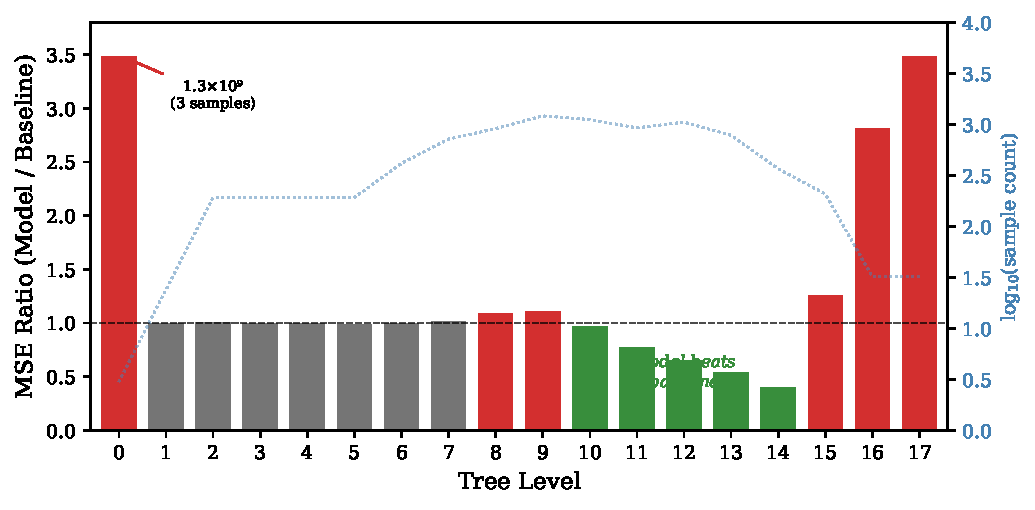
\includegraphics[width=\columnwidth]{figures/fig2_per_level_mse.pdf}
  \caption{Per-level MSE ratio (model/baseline) on the validation set. The model beats $\rho_0$ at levels 10--14 (ratio $< 1$) but matches or slightly exceeds it at coarse levels 1--9 (ratio $\geq 1$). Levels 0, 15--17 have too few training samples for reliable prediction.}
  \label{fig:per_level_mse}
\end{figure}

After applying level-aware masking (hard
cutoff below 200 training samples, $\sqrt{n/n_\text{max}}$ sample
weighting), the model beat $\rho_0$ at fine levels and matched it at
coarse levels:
%
\begin{itemize}
  \item Level 0 (3 samples): $1.34 \times 10^{9}\times$ baseline.
        Catastrophic failure from extreme data scarcity, masked during
        training but exposed at inference.
  \item Levels 1--9 (24--1216 samples): $1.00$--$1.12\times$.
        Near-parity with $\rho_0$.
  \item Level 10 (1120 samples): $0.98\times$.
  \item Level 11 (928 samples): $0.79\times$.
  \item Level 12 (1056 samples): $0.67\times$.
  \item Level 13 (784 samples): $0.55\times$.
  \item Level 14 (368 samples): $0.41\times$.
  \item Level 15 (208 samples): $1.27\times$.
        Performance degrades as sample counts drop below the masking
        threshold.
  \item Levels 16--17 (32 samples each): $2.83\times$ and $5.34\times$.
\end{itemize}
%
The model learns a genuine correction to $\rho_0$ at levels 10--14,
where training data is abundant and the density correction signal is
spatially localized near nuclei. At coarser levels, the correction
is a non-local function of electron-electron interactions that cannot
be inferred from same-level halo features alone.

We constructed a level-clamped predictor that uses the ML model at
levels 10--14 and falls back to $\rho_0$ elsewhere. This hybrid
achieved an aggregate validation MSE of $0.97\times$ baseline: a 3\%
improvement over $\rho_0$. The natural question is whether this
improvement translates to fewer SCF iterations.

\subsection{Parent Node Features}
\label{sec:parent_features}

One hypothesis for the coarse-level plateau is that the model lacks
multi-resolution context. To test this, we concatenated parent-node
$\rho_0$ and $V_\text{nuc}$ s-coefficients (1024 additional floats per
sample) to the trunk input, increasing it from 1792 to 2816 dimensions
and total parameters from 3.0M to 4.1M. Because the first layer shape
changed, we trained from scratch rather than fine-tuning.

The result was negative. Per-level MSE ratios were identical to those
of the model without parent features, within training noise. The parent
$\rho_0$ and $V_\text{nuc}$ encode the same atomic superposition signal
at coarser resolution. They do not contain the density correction
(exchange-correlation, orbital relaxation, bonding redistribution)
because that correction is what the converged SCF procedure computes.
Adding a coarser copy of the input does not introduce new information
about the target.

\subsection{SCF Convergence Test}
\label{sec:scf_test}

We injected the level-clamped density into MADNESS and ran full SCF
calculations on 7 molecules at two convergence thresholds ($10^{-6}$
and $10^{-8}$), yielding 14 comparisons against the $\rho_0$ baseline
(\autoref{tab:scf_iterations}).

\begin{table}[htbp]
\centering
\caption{SCF iteration counts for level-clamped ML density (levels 10--14) vs.\ promolecular baseline ($\rho_0$). All 14 comparisons yield identical iteration counts. Ground-state energies agree to 8+ significant figures.}
\label{tab:scf_iterations}
\begin{tabular}{lccrrc}
\toprule
Molecule & $N_e$ & Thresh & Baseline & ML & $E_\text{base}$ (Ha) \\
\midrule
CH$_3$OH & 18 & $10^{-6}$ & 12 & 12 & -114.85038034 \\
CH$_3$OH & 18 & $10^{-8}$ & 12 & 12 & -114.85038034 \\
Ethanol & 26 & $10^{-6}$ & 12 & 12 & -153.81559584 \\
Ethanol & 26 & $10^{-8}$ & 12 & 12 & -153.81559584 \\
SO$_2$ & 32 & $10^{-6}$ & 14 & 14 & -546.34469275 \\
SO$_2$ & 32 & $10^{-8}$ & 14 & 14 & -546.34469265 \\
HN$_3$ & 22 & $10^{-6}$ & 13 & 13 & -163.57199524 \\
HN$_3$ & 22 & $10^{-8}$ & 13 & 13 & -163.57199524 \\
H$_2$O$_2$ & 18 & $10^{-6}$ & 12 & 12 & -150.55376660 \\
H$_2$O$_2$ & 18 & $10^{-8}$ & 12 & 12 & -150.55376660 \\
C$_2$H$_2$ & 14 & $10^{-6}$ & 10 & 10 & -76.63064903 \\
C$_2$H$_2$ & 14 & $10^{-8}$ & 10 & 10 & -76.63064903 \\
Glyoxal & 30 & $10^{-6}$ & 13 & 13 & -226.15979738 \\
Glyoxal & 30 & $10^{-8}$ & 13 & 13 & -226.15979738 \\
\bottomrule
\end{tabular}
\end{table}


All 14 comparisons produced identical iteration counts. CH$_3$OH
converged in 12 iterations with both initial guesses. Ethanol: 12.
SO$_2$: 14. HN$_3$: 13. H$_2$O$_2$: 12. C$_2$H$_2$: 10.
Glyoxal: 13. Ground-state energies agreed to 8 or more significant
figures (e.g., $E_{\text{CH}_3\text{OH}} = -114.85038034$ Ha for the
baseline vs.\ $-114.85038032$ Ha for the ML density). The correct
electronic state was recovered in every case.

The mechanism is straightforward. MADNESS uses a multi-protocol SCF
strategy: the first protocol solves at a coarse threshold
($\epsilon = 10^{-4}$), and subsequent protocols refine progressively.
The coarse protocol sets the density at levels 1--9, which determines
the convergence path. Fine-level improvements at levels 10--14, where
the ML model outperforms $\rho_0$, are projected away when the tree is
compressed to the coarse threshold. By the time later protocols operate
at fine resolution, the density has already been updated by SCF
iterations and the initial guess is irrelevant.

Tightening the final threshold from $10^{-6}$ to $10^{-8}$ does not
change this conclusion. The additional refinement occurs at even finer
levels, but the coarse-level convergence path remains identical.

\subsection{Tree Structure Prediction}
\label{sec:tree_prediction}

The density prediction results suggest that the local receptive field
limits regression accuracy at coarse levels. We tested whether the same
limitation applies to a simpler task: predicting which nodes require
adaptive refinement (a binary classification problem).

Multi-task training (density regression + refinement classification)
achieved F1 = 0.857. The learned $\sigma_{\rho_s}$ shrank to 0.075,
upweighting the density loss by 89$\times$ and starving the refinement
classification head. Training the refinement head alone with focal
loss~\cite{lin2017focal} ($\gamma = 2$, $\alpha = 0.75$) yielded
F1 = 0.860, a delta of 0.003. Removing multi-task interference had
negligible effect on the classification ceiling.

We tested the refine-only model in an SCF tree-walk: starting from
the ML-predicted tree structure rather than the $\rho_0$ tree.
CH$_3$OH required 31 iterations compared to 12 with the baseline
tree, a factor of 2.6$\times$ worse. The model did recover the
correct electronic state (energies agreed to 7 significant figures:
$-114.85038034$ vs.\ $-114.85037863$ Ha), confirming that the SCF
procedure corrects the tree errors at the cost of additional
iterations.

The classification task faces the same receptive field limitation
as regression. Whether a node at level $N$ should be refined depends
on the density structure at levels 0 through $N-1$, which determines
the wavelet coefficients that trigger refinement in MADNESS. A model
restricted to same-level halo neighbors cannot access this information.

\section{Analysis}
\label{sec:analysis}

The experiments in Section~\ref{sec:results} present a consistent picture:
the model learns a genuine correction to $\rho_0$ at fine tree levels
(10--14) but cannot improve on the promolecular density at coarse levels
(1--9). Since the coarse levels determine SCF convergence, the fine-level
improvement has no effect on iteration count. This section explains why.

MADNESS solves the Kohn--Sham equations~\cite{kohn1965self} through a
multi-protocol SCF strategy~\cite{harrison2016madness}. The first
protocol operates at a coarse truncation threshold
($\epsilon = 10^{-4}$), which resolves only tree levels 1 through
approximately 9. At this threshold, the adaptive tree discards all
structure below the coarse truncation scale: wavelet coefficients at
levels 10--14 fall below $\epsilon$ and are projected away when the Fock
matrix is constructed. The SCF cycle at this coarse protocol determines
the number of iterations required and the electronic state reached. Once
the coarse protocol converges, subsequent protocols inherit the
converged coarse density and refine it by adding spatial detail at
progressively finer levels. These later protocols do not revisit the
coarse-level convergence path. They begin from a density that is already
self-consistent at the coarse scale and simply resolve additional spatial
structure (Figure~\ref{fig:tree_schematic}).

\begin{figure}[htbp]
  \centering
  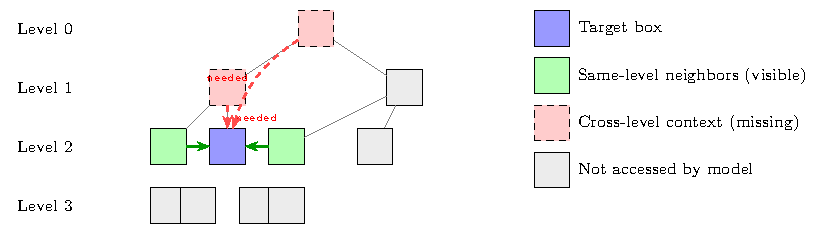
\includegraphics[width=\columnwidth]{figures/fig4_tree_schematic.pdf}
  \caption{Receptive field limitation of the halo-neighbor architecture. The model at a target node (blue) sees only same-level face-adjacent neighbors (green). Cross-level context from parent and root nodes (red, dashed) is needed to capture the global electronic structure that determines the density correction at coarse levels.}
  \label{fig:tree_schematic}
\end{figure}

This multi-protocol structure explains the SCF test results directly.
The level-clamped predictor improves on $\rho_0$ only at levels 10--14.
When MADNESS compresses the initial guess to the first-protocol
threshold, these improvements vanish. The coarse-level density seen by
the first SCF protocol is identical whether the initial guess is
$\rho_0$ or the ML-corrected density. The iteration counts match because
the two initial guesses are, at the resolution that matters,
indistinguishable.

The question then becomes: why does the model fail at coarse levels?
The answer lies in what the input features encode and what the target
correction requires. At any tree level, $\rho_0$ is a smooth
superposition of spherically symmetric atomic densities. $V_\mathrm{nuc}$
is the nuclear Coulomb potential. Both are functions of atomic positions
and species alone. The target correction
$\Delta\rho = \rho_\mathrm{conv} - \rho_0$ encodes
exchange-correlation effects, orbital relaxation, and the redistribution
of electron density due to chemical bonding. These are consequences of
the full many-electron wavefunction. They arise from non-local
electron-electron interactions that the self-consistent field procedure
computes iteratively by solving the Kohn--Sham eigenvalue problem over
the entire molecular domain.

At fine levels (10--14), the correction $\Delta\rho$ is spatially
localized near nuclei and varies smoothly as a function of the local
atomic environment. Same-level halo neighbors provide enough context for
the model to interpolate this correction from training data. At coarse
levels, $\Delta\rho$ reflects global electronic structure: how orbitals
delocalize across the molecule, how exchange-correlation modifies the
density at scales comparable to bond lengths, and how the occupied
orbital space responds to the full molecular potential. The input
features at a coarse node, consisting of $\rho_0$ and $V_\mathrm{nuc}$
at that node and its six face-adjacent neighbors, do not contain this
information and cannot contain it. The promolecular density and nuclear
potential at a handful of neighboring boxes encode atomic positions and
charges, not the self-consistent electronic response to those charges.

This is not a model capacity problem. The parent feature experiment
(Section~\ref{sec:parent_features}) increased parameters from 3.0M to
4.1M with no change in coarse-level accuracy. It is not a data
problem. Expanding the training set from 15 to 51 molecules improved
fine-level predictions but left coarse-level ratios unchanged at
1.00--1.12$\times$ baseline. It is an input sufficiency problem: the
mapping from $(\rho_0, V_\mathrm{nuc})$ to $\Delta\rho$ at coarse
levels is not a well-defined function of those inputs. Multiple
distinct corrections $\Delta\rho$ can arise from the same local
$\rho_0$ and $V_\mathrm{nuc}$ pattern, because the correction depends
on the global molecular context that the local inputs do not resolve.

Could a different architecture overcome this limit? The parent feature
experiment tested the simplest form of multi-scale context: concatenating
the $\rho_0$ and $V_\mathrm{nuc}$ coefficients from the parent node.
This expanded the receptive field to span two tree levels, but the
additional information was a coarser copy of the same signal. A graph
neural network or attention-based architecture that aggregates
information across the entire tree would have access to every node in
the adaptive representation. However, if the node-level features remain
$\rho_0$ and $V_\mathrm{nuc}$, then global aggregation produces a
summary of the promolecular density and nuclear potential, not of the
self-consistent density. The quantity the model needs to predict, the
electron-electron interaction correction, is precisely what is absent
from these inputs. No aggregation scheme over $\rho_0$ and
$V_\mathrm{nuc}$ can reconstruct $\Delta\rho$ at coarse levels, because
$\Delta\rho$ is not a function of $\rho_0$ and $V_\mathrm{nuc}$ alone.
It depends on the solution of the Kohn--Sham equations, which is the
output of the SCF procedure, not a property of the input potential.

This is the fundamental limit. A local ML model that takes the
promolecular density and nuclear potential as input and produces a
density correction as output is attempting to bypass the SCF iteration
by learning its fixed point from input data that does not determine
that fixed point. The model succeeds at fine levels because there the
fixed-point correction happens to be a smooth, spatially localized
function that correlates with the local atomic environment. It fails
at coarse levels because there the correction is a global property of
the electronic state. The multi-protocol SCF structure of MADNESS then
ensures that only the coarse-level result affects convergence speed.
The fine-level success, while real, is operationally irrelevant.

\section{Lessons and Path Forward}
\label{sec:lessons}

Three observations from this work generalize beyond the MRA-NN setting
and may inform future attempts to couple ML models with iterative
scientific solvers.

Input signal quality determines the ceiling of any downstream model,
independent of architecture capacity. Our parent model doubled the
input dimension (2816 vs.\ 1792 features) and added 34\% more
parameters (4.1M vs.\ 3.0M), yet reproduced the per-level MSE ratios
of the base model almost exactly. The single-task ablation confirmed
that multi-task interference was a real training pathology, but
removing it only brought the model to parity with $\rho_0$, not beyond
it. The fundamental limitation is that the promolecular density and
nuclear potential carry no electron-electron correlation signal. No
amount of nonlinear capacity can extract exchange-correlation physics
from inputs that do not encode it.

Fine-scale accuracy does not imply solver acceleration. The level-clamped
model achieved MSE ratios of 0.41--0.98$\times$ baseline at levels
10--14, a measurable and statistically significant improvement over
$\rho_0$. Yet SCF injection tests produced identical iteration counts
across all 14 molecule-threshold combinations (7 molecules, 2
thresholds). The explanation is structural: MADNESS
protocols~\cite{harrison2016madness} refine from coarse to fine,
and iteration count is determined by the coarsest protocol stage
where the initial density deviates from the converged solution.
Improvements at spatial scales finer than the first protocol
threshold provide no leverage on convergence. Any ML model targeting
solver acceleration must improve the density at the resolution the
solver actually queries first, not at the resolution where data is
most abundant.

Multi-task interference in uncertainty-weighted losses can silently
undermine the primary objective. Kendall uncertainty
weighting~\cite{kendall2018multitask} allowed the learned scale
parameter $\sigma_{\rho_s}$ to grow without bound, progressively
zeroing the density gradient while the classification head consumed
the entire learning signal. The resulting model was 2.99$\times$
worse than $\rho_0$ on density prediction, yet the aggregate loss
decreased monotonically, masking the failure. A subsequent
configuration flag (\texttt{refine\_focused}) appeared to fix this
by switching the checkpoint selection metric to refinement F1, but it
left the loss function unchanged; the density head still trained under
the corrupted gradient. Refine-only training with pure focal loss
achieved F1\,=\,0.860, a gain of only 0.003 over the multi-task
formulation (F1\,=\,0.857). The broader warning is that multi-task
losses with learned weighting parameters require per-head monitoring
of both loss and scale; aggregate convergence is not a reliable
diagnostic.

\subsection{Path Forward: Gaussian-Basis Density as ML Input}
\label{sec:path_forward}

The negative results above point to a concrete next step. If the
bottleneck is input signal quality, the remedy is to supply an input
that already contains exchange-correlation physics. A natural candidate
is the converged density from a Gaussian-basis DFT calculation (e.g.,
Dalton), projected onto the MRA grid. Preliminary experiments by
collaborators show that using the Dalton density directly as the
MADNESS starting guess reduces SCF iteration counts, confirming that
the missing signal is the core issue.

This reframes the ML problem from predicting a large correction
(promolecular $\rho_0$ $\to$ converged MRA $\rho$) to predicting a
small residual (Gaussian-basis $\rho_{\text{GTO}}$ $\to$ converged MRA
$\rho$). The residual is dominated by basis-set truncation artifacts
near nuclei and in diffuse tails, both of which are spatially localized
and well-suited to the local halo-feature architecture already
developed. We plan to construct training data by pairing Dalton
densities with converged MADNESS densities for the same molecules and
to retrain the single-task model on the resulting residuals. No
results from this approach are available yet, and the magnitude of the
achievable speedup remains an open question.

\section{Conclusion}
\label{sec:conclusion}

We trained three local ML models to accelerate SCF convergence in
MADNESS and all three failed. A level-clamped density predictor achieved
MSE ratios of 0.41--0.98$\times$ baseline at fine tree levels (10--14)
and 1.00--1.12$\times$ at coarse levels (1--9), producing identical SCF
iteration counts across all 14 molecule-threshold combinations.
A parent-node feature model expanded the architecture to 4.1M parameters
and doubled the input dimension, yet reproduced the same per-level MSE
ratios as the base model, confirming that additional capacity extracts no
new signal from the available inputs. A tree structure predictor reached
F1\,=\,0.860 but required 31 SCF iterations versus 12 for the
promolecular guess, a 2.6$\times$ degradation.

The common root cause is an input signal bottleneck at coarse tree
levels. MADNESS converges its SCF solution at levels 1--9 before
refining finer scales, so only coarse-level density corrections can
reduce iteration counts. The promolecular density and nuclear potential
at those levels encode atomic superposition and electrostatics but carry
no electron-electron interaction information. No local model operating on
these inputs can produce the exchange-correlation corrections needed to
improve the coarse-level density, regardless of architecture or training
procedure.

This mechanistic explanation (that multi-scale solvers gate convergence
at their coarsest resolution, where atom-centered inputs lack the
relevant physics) is not specific to MADNESS or to density functional
theory. It applies whenever an ML model receives only single-body inputs
and targets a quantity governed by many-body interactions, and the
iterative solver queries coarse scales first. Recognizing this pattern
before training avoids the cycle of architecture search and
hyperparameter tuning that preceded our diagnosis.

One path remains open. A converged Gaussian-basis density already
contains exchange-correlation physics and, when used directly as a
MADNESS starting guess, reduces SCF iteration counts. An ML model
trained on the small residual between the Gaussian-basis density and the
converged MRA density would operate on an input that does not suffer from
the signal bottleneck identified here. Whether this residual is
learnable with local features, and whether the resulting speedup
justifies the cost of the Gaussian-basis calculation, are questions that
require new experiments.


\begin{acknowledgement}
% TODO: funding acknowledgements
\end{acknowledgement}

\bibliography{references}

\end{document}
